\chapter{Ausblick}

Der Ausblick umfasst die Betrachtung von möglichen Verbesserungen der Simulationen und technische Entwicklungen, die in naher Zukunft für ein kommunales Inselnetz wirtschaftlich seien könnten.
Eine Zusammenführung der bilanziellen und dreiphasigen Simulation in ein MatLab/Simulink-Modell ist wünschenswert, aufgrund der hohen Simulationszeit des bilanziellen Systems jedoch nur mit unproportionalem Zeitaufwand möglich.
Die simulierte Zeit pro Sekunde sollte dafür vom Verhältnis von ungefähr 1:1 auf 60:1 verbessert werden.
Generell sind bei beiden Simulationsmodellen im Aufbau viele Komponenten und Einflüsse vereinfacht worden. 
Um eine realistischere Simulation zu erhalten, können diese genauer abgebildet werden.
Bei den Stromerzeugern können Photovoltaikanlagen der Simulation hinzugefügt werden.
Anhand von Faktoren wie dem Material der Solarzellen, dem Wirkungsgrad, installierter Leistung, Systemverlust, Neigung und Azimut, sowie Daten für die Solareinstrahlung des Standortes der Kommune kann ein komplexes Modell dieses Erzeugers in MatLab/Simulink erstellt werden\cite{jrcpv}.
Die Implementation des Erzeugers PV würde, da dieser sonneneinstrahlungsabhängig ist, zu einer komplexeren Fluktuation bei der Stromerzeugung im Netz führen. 
Dies hat generellen Einfluss auf das Netz und die Dimensionierung, als auch Be- und Entladestrategien von Speichern.
Weitere erneuerbare Energien, die betrachtet werden können sind Gezeiten- und Wasserkraft (s. Abbildung).
Die Auswahl dieser regenerativen Energiequellen ist jedoch stark von der geographischen Lage des Inselnetzes abhängig.
  
\begin{figure}[h!]
    \centering
    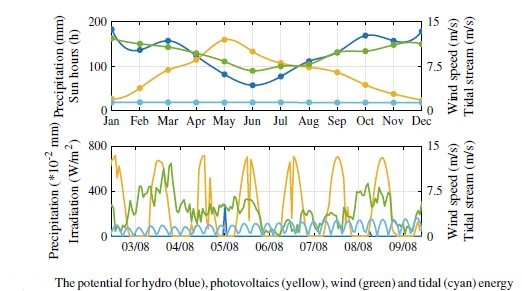
\includegraphics[width=14cm]{Abbildungen/AusblickAbb1.jpg}
    \caption{Betrachtung potentieller erneuerbarer Stromerzeuger für das Fallbeispiel Färöer-Inseln\cite{faroer}}\label{fig:Stromerzeuger_Faroer}
\end{figure}

Außerdem kann die Modellierung eines Prosumers, bestehend aus einem Haus mit Wärmepumpe, PV-Anlage und Speicher, am Netz betrachtet werden.
Die Modellierung ist hierbei komplex und deren Auswirkungen für das Netz können relevant sein.
Ursache dafür ist die Komplexität dieses Subsystem des Inselnetzes.
Bei einem solchen Prosumer liegt ein Zusammenspiel von PV-Anlage und internem Speicher zugrunde.
Für diesen können eigene Be- und Entladestrategien betrachtet werden, die außerdem neben dem allgemeinen Strombedarf des Hauses noch mit dem Strombedarf einer angeschlossenen Wärmepumpe zusammenspielen.
Durch die Abhängigkeit des Heizverhaltens der Wärmepumpe von der Außentemperatur, aus welcher sich der Heizbedarf ermitteln lässt, entsteht zusammenfassend eine in sich komplexe Komponente im Modell.
Ein weiterer Verbrauchsfaktor für ein Inselnetz ist die E-Mobilität.
Hierbei stehen die Betrachtung und ggf. Steuerung des Ladeverhaltens der E-Fahrzeuge im Vordergrund.
Darüber kann die Interkation von privaten E-Fahrzeugen mit privaten Stromspeichern aus dem Modell des beschriebenen Prosumers simuliert werden.
Auch bei den Speichersystemen sind Änderungen implementierbar.
In beiden Modellen werden ausschließlich Batteriespeichersysteme modelliert.
Eine Simulation eines Fernwärmenetzes als auch die Nutzung von Power-to-Gas und Gas-to-Power sind möglicher Erweiterungen für die Modelle.
Die existierenden Batteriemodelle können auch präziser modelliert werden.
Dabei ist die Betrachtung von elektrischen Batteriemodellen ein möglicher Schritt, der es ermöglichen würde, elektrische Phänomene im Netz genauer zu betrachten.
Dadurch können gleichzeitig die Aufgaben von Batteriespeichersystemen umfassender simuliert werden.
Außerdem können in einer erweiterten Simulation auf Dauer weitere relevante Faktoren implementiert werden, beispielsweise ein Peak Shaving Algorithmus.
Eine Darstellung von Redox-Flow-Batteriespeichern findet außerdem auch nicht statt, ist aber möglich und sinnvoll, insbesondere wenn ebendiese wirtschaftlich und technisch eine Alternative zu Lithium-Ionen-Batteriespeichern darstellen.
Für die bilanzielle Simulationen wäre eine Erweiterung der Simulation wünschenswert, bei die Betrachtung von elektrischen Phänomenen allgemein möglich ist. 
Jedoch darf die Simulationsgeschwindigkeit dadurch nicht stark beeinträchtigt werden.
Bei der Modellierung des dreiphasigen Inselnetzes gibt es mehrere Erweiterungsoptionen. 
Die Implementierung einer Ladestrategie für die Windkraftspeicher kann die Qualität der Simulation verbessern.
Darüber hinaus ist in Anbetracht der gewünschten Nutzung von ausschließlich erneuerbaren Erzeugern die Entfernung des Dieselgenerators eine Möglichkeit.
Dies ist allerdings nur umsetzbar, wenn im gleichen Zug eine Implementierung einer Frequenzmessung stattfindet, da der Dieselgenerator essentiell für diese Messung ist.
Darüber hinaus ist die Betrachtung der Blindleistung im Modell implementierbar.
Allgemein können auch Prognosen im Bereich der Strombedarfsermittlung und der Veränderung von Verbrauchern einen Mehrwert für die Modellierung darstellen.
Das liegt daran, dass im Zuge der Abkehr von fossilen Energieträgern insbesondere in den Bereichen Gewerbe, Industrie und Verkehr damit zu rechnen ist, dass ein Großteil des Energiebedarfes in Deutschland und vielen anderen Teilen der Welt auf Dauer durch Strom gedeckt werden soll.
Die resultierende momentane Entwicklung spielt dabei eine ausschlaggebende Rolle und die technische Weiterentwicklung, insbesondere im Bereich der Speichertechnologien, prägt den Aufbau und die Veränderung jedes Stromnetzes.


\chapter{Fazit}
